\subsection{Skenario Pengujian}
\begin{frame}{Skenario Pengujian}
  Terdapat dua skenario yang akan diuji untuk membandingkan teknik-teknik yang telah disebutkan.
  \begin{itemize}
    \item Pelatihan model sederhana untuk mempelajari dataset Fashion-MNIST \parencite{xiao2017fashion}.
    \item Pelatihan ResNet-20 untuk mempelajari dataset CIFAR10 \parencite{krizhevsky2009cifar}.
  \end{itemize}
\end{frame}

\subsubsection{Fashion-MNIST}
\begin{frame}{Fashion-MNIST}
  \begin{itemize}
    \item Fashion-MNIST \parencite{xiao2017fashion} adalah suatu \textit{dataset} yang berisi 60000 gambar pakaian berukuran 28 $\times$ 28 piksel dari Zalando.

    \item Akan digunakan model sederhana untuk melakukan klasifikasi. Arsitektur model dapat dilihat pada gambar berikut.
  \end{itemize}
  \begin{figure}
    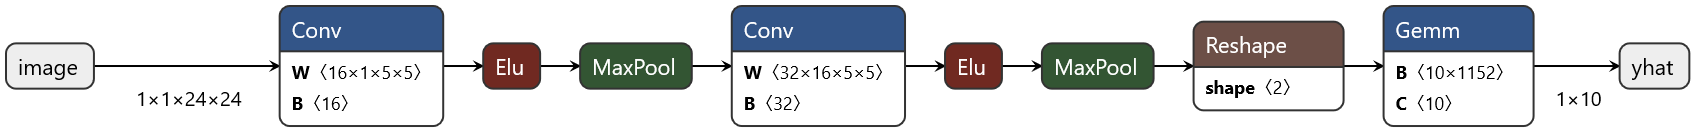
\includegraphics[width=13cm]{fashion_mnist.onnx.png}
    \caption{Model sederhana untuk klasifikasi Fashion-MNIST}\label{modelfashion}
  \end{figure}
\end{frame}

\begin{frame}{Hyperparameter}
  \begin{columns}[b]
    \begin{column}{3.5cm}
      Hyperparameter untuk CADA \\
      \vspace{1cm}
      \begin{tabular}{ | c | c | }
        \hline
        \textbf{Parameter} & \textbf{Nilai} \\
        \hline
        $\alpha$           & 0.00001        \\
        \hline
        $\beta_1$          & 0.9            \\
        \hline
        $\beta_2$          & 0.99           \\
        \hline
        $D$                & 50             \\
        \hline
        $d_{max}$          & 10             \\
        \hline
        $c$                & 400            \\
        \hline
      \end{tabular}
    \end{column}
    \begin{column}{3.5cm}
      Hyperparameter untuk Efficient-Adam \\
      \vspace{1cm}
      \begin{tabular}{ | c | c | }
        \hline
        \textbf{Parameter} & \textbf{Nilai} \\
        \hline
        $\alpha$           & 0.0001         \\
        \hline
        $\beta_1$          & 0.9            \\
        \hline
        $\beta_2$          & 0.999          \\
        \hline
      \end{tabular}
    \end{column}
    \begin{column}{3.5cm}
      Hyperparameter untuk gabungan \\
      \vspace{1cm}
      \begin{tabular}{ | c | c | }
        \hline
        \textbf{Parameter} & \textbf{Nilai} \\
        \hline
        $\alpha$           & 0.0001         \\
        \hline
        $\beta_1$          & 0.9            \\
        \hline
        $\beta_2$          & 0.99           \\
        \hline
        $D$                & 50             \\
        \hline
        $d_{max}$          & 10             \\
        \hline
        $c$                & 400            \\
        \hline
      \end{tabular}
    \end{column}
  \end{columns}
\end{frame}

\subsubsection{CIFAR10}
\begin{frame}{CIFAR10}
  \begin{itemize}
    \item CIFAR10 \parencite{krizhevsky2009cifar} merupakan dataset yang berisi 60.000 gambar berwarna berukuran 32 $\times$ 32 piksel. Seluruh gambar diklasifikasi ke dalam 10 kelas yang berbeda.
    \item Akan digunakan model ResNet-20 \parencite{Idelbayev18a} untuk melakukan klasifikasi terhadap dataset CIFAR10. Model ResNet memiliki \textit{building block} berupa \textit{residual block} yang diilustrasikan pada gambar di bawah.
  \end{itemize}
  \begin{figure}
    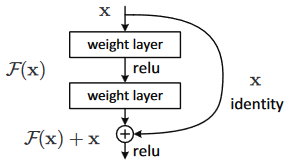
\includegraphics{resblock.png}
    \caption{Blok residu dalam ResNet \parencite{Idelbayev18a}}
  \end{figure}
\end{frame}

\begin{frame}{Hyperparameter}
  \begin{columns}[b]
    \begin{column}{3.5cm}
      Hyperparameter untuk CADA \\
      \vspace{1cm}
      \begin{tabular}{ | c | c | }
        \hline
        \textbf{Parameter} & \textbf{Nilai} \\
        \hline
        $\alpha$           & 0.01           \\
        \hline
        $\beta_1$          & 0.9            \\
        \hline
        $\beta_2$          & 0.99           \\
        \hline
        $D$                & 50             \\
        \hline
        $d_{max}$          & 2              \\
        \hline
        $c$                & 0.12           \\
        \hline
      \end{tabular}
    \end{column}
    \begin{column}{3.5cm}
      Hyperparameter untuk Efficient-Adam \\
      \vspace{1cm}
      \begin{tabular}{ | c | c | }
        \hline
        \textbf{Parameter} & \textbf{Nilai} \\
        \hline
        $\alpha$           & 0.0005         \\
        \hline
        $\beta_1$          & 0.9            \\
        \hline
        $\beta_2$          & 0.999          \\
        \hline
      \end{tabular}
    \end{column}
    \begin{column}{3.5cm}
      Hyperparameter untuk gabungan \\
      \vspace{1cm}
      \begin{tabular}{ | c | c | }
        \hline
        \textbf{Parameter} & \textbf{Nilai} \\
        \hline
        $\alpha$           & 0.0005         \\
        \hline
        $\beta_1$          & 0.9            \\
        \hline
        $\beta_2$          & 0.999          \\
        \hline
        $D$                & 50             \\
        \hline
        $d_{max}$          & 2              \\
        \hline
        $c$                & 0.12           \\
        \hline
      \end{tabular}
    \end{column}
  \end{columns}
\end{frame}
